% Six-page conference version. Every number is taken from the long paper
% (paper/main.tex) and the results files it names; nothing here is measured only here.
\documentclass[conference]{IEEEtran}
\usepackage[T1]{fontenc}
\usepackage{graphicx}
\usepackage{booktabs}
\usepackage{amsmath}
\usepackage{cite}
\usepackage{url}
\graphicspath{{../figures/}{figures/}}

\begin{document}

\title{Recording Domain, Not Code-Mixing: Closing the Generalisation Gap of\\
Audio Deepfake Detection on Hindi--English Telephone Speech}

\maketitle

\begin{abstract}
Deepfake detectors report error rates below one percent on English benchmarks.
We test what that means for Hindi--English speech over a telephone line. A
wav2vec~2.0 detector trained on ASVspoof 2019 LA
reaches 0.85\% equal error rate on English but 58.42\% on code-mixed speech over a
simulated narrowband channel; it rejects genuine speakers, calling 94.8\% of clean genuine
Hindi--English speech fake. A language-controlled
test on 183 unseen speakers shows the gap follows the recording domain, not
code-mixing. Low-rank adaptation of 1.13\% of the parameters brings channel-matched error to
2.75\% (the deployed model). More training speakers and a real codec help most: the final
recipe, trained on 248 speakers over simulated G.711 and real AMR-NB, takes error on new
speakers' unseen Tortoise clones from 30.8\% to 8.8\% over the line and from 36.3\% to 6.0\%
over AMR-NB across five seeds, with no unseen-tool audio in training. A larger encoder
(SSL-AASIST) fine-tuned on the same data reaches 0.5\% over AMR-NB and 12.9\% on Chatterbox,
another unseen generator. The main results are tested against a shortcut floor of cheap
signal statistics by a paired speaker bootstrap. Spontaneous speech, IndicF5 and, for the adapters, Chatterbox
remain unsolved. The detector runs on live calls, warning only the callee. On 30 real mobile
calls scored offline, the deployed model, failing mostly at the mobile codec, warns most
genuine live calls, the final recipe one in four, and flags five of six seen-tool clone calls as
likely cloned.
\end{abstract}

\begin{IEEEkeywords}
audio deepfake detection, anti-spoofing, code-mixing, telephone channel, low-rank adaptation
\end{IEEEkeywords}

\section{Introduction}

Voice cloning is now a consumer product. A few seconds of someone's speech are enough for
a zero-shot system to say new sentences in that person's voice~\cite{casanova2024xtts,
betker2023tortoise}, and voice conversion does the same without a
transcript~\cite{rvc2023}. The obvious criminal use is a phone call: a familiar voice
asking for money or a one-time code.

Detection research has strong numbers to show. On ASVspoof 2019 LA~\cite{todisco2019asvspoof},
detectors that fine-tune a self-supervised speech encoder reach error rates below one
percent~\cite{tak2022wav2vec}, and our wav2vec~2.0 detector trained on the same benchmark
reaches 0.85\% EER. That figure is
measured on English studio speech. In India, many of the people who receive these calls
speak code-mixed Hindi and English, switching language inside a single sentence, and they
hear the caller through a narrowband telephone channel. We ask what happens to a detector
when both conditions change at once, why it happens, and what it costs to fix.

The answer to the first question is stark. The English detector fails, and it fails by
rejecting real speakers rather than by missing clones. The answer to the second is less
obvious. The natural suspect is the language mix, but when we hold speaker and recording
fixed and change only the language, the detector rejects genuine English at least as often
as code-mixed speech. The gap follows the recording domain.

A low error rate on a newly built corpus can also be obtained for the wrong reason. Real
and cloned clips that differ in loudness or bandwidth can be told apart without any
knowledge of speech synthesis. We therefore compare every code-mixed EER of the systems we
adapt with a shortcut floor fitted on the same training data and scored on the same clips. Our
contributions are:
\begin{itemize}
\item a measured gap on Hindi--English telephone speech, traced by a language-controlled
test of 183 unseen speakers to the recording domain rather than to code-mixing;
\item closure of the gap by low-rank adapters~\cite{hu2022lora} on a frozen wav2vec~2.0
encoder~\cite{baevski2020wav2vec}, which, added to the English detector, keep clean English
in the deployed configuration (2.42\%; the final recipe keeps less, 13.44\%);
\item evidence that more training speakers (genuine speech and seen-tool clones of them) and
a real mobile codec, with no new attack tool,
close most of the remaining gap on the unseen Tortoise generator, over five training seeds
and with a larger encoder, while IndicF5 and Chatterbox stay hard;
\item matched shortcut floors with a paired speaker bootstrap for our systems, which
changed several of our own conclusions; and
\item a live-call system that runs the same detector, at an operating point calibrated on
development calls, warns only the person receiving the call, and has a first test on real
mobile calls.
\end{itemize}

\section{Related work}

\textbf{Benchmarks and generalisation.} ASVspoof 2019 LA~\cite{todisco2019asvspoof} is
English studio speech with text-to-speech and voice conversion attacks, and ASVspoof
2021~\cite{liu2023asvspoof2021} added telephony codecs and compressed audio. Detectors
trained on ASVspoof degrade sharply on audio collected in the
wild~\cite{muller2022generalize}. End-to-end systems such as RawNet2~\cite{tak2021rawnet2}
and AASIST~\cite{jung2022aasist} learn from the raw waveform; the strongest recent recipes
fine-tune a self-supervised encoder such as wav2vec~2.0 or
XLS-R~\cite{baevski2020wav2vec,babu2022xlsr} with RawBoost
augmentation~\cite{tak2022rawboost,tak2022wav2vec}.

\textbf{Channels and codecs.} Telephony is usually handled by augmentation, with
companding~\cite{das2021companding} or with landline, cellular and VoIP codecs sampled
during training~\cite{chen2021channel}. Tsutsumi et al.~\cite{tsutsumi2026channel} find
countermeasures near chance on real phone and VoIP recordings and recover by adapting to
degraded in-domain speech, and Delgado et al.~\cite{delgado2026presentation} argue that
detectors fail in deployment because training audio never passes through the presentation
channel. RTCFake~\cite{xue2026rtcfake} passes deepfakes through conferencing platforms such
as Zoom; we target narrowband telephone codecs.

\textbf{Parameter-efficient adaptation.} LoRA~\cite{hu2022lora} has been applied to
wav2vec~2.0 fake-audio detection, where it matches full fine-tuning with far fewer
trainable parameters~\cite{wang2023lora}. We use it for a different reason: added to an
English detector, it learns code-mixed speech while our deployed detector keeps clean
English.

\textbf{Multilingual and code-switched detection.} MLAAD~\cite{muller2024mlaad} and
SpeechFake~\cite{huang2025speechfake} span many languages,
IndicSynth~\cite{sharma2025indicsynth} covers twelve Indian languages, and
Indic-CodecFake~\cite{girish2026indiccodecfake} and SEA-CF~\cite{phukan2026seacf} show
English-trained detectors failing on Indic and South-East Asian speech. These corpora hold
one language per utterance. Switching inside an utterance has been studied for
Arabic--English in an audio-visual setting~\cite{kuckreja2026habibi} and for
Vietnamese--English in the VietPrism corpus~\cite{hoang2026vietprism}. We found no
detection study of Hindi--English code-mixing, in audio, evaluated over a telephone
channel.

\section{Data}

\subsection{Speech and speaker pools}

Genuine code-mixed speech comes from MUCS 2021 Hindi--English~\cite{diwan2021mucs}: 52,825
clips, 89.5 hours and 520 speakers of lecture and read speech. HiACC adds 3,318 clips of
spontaneous speech from 24 adult speakers, used for evaluation only; its child recordings
(1,858 of 5,176 files) are excluded from every use. English comes from ASVspoof 2019 LA.

MUCS speakers were divided into disjoint pools before any audio was cloned, so no pool
could be chosen after seeing which voices clone well: 25 speakers for attack training, 10
for adaptation (8 for training, 2 for development) and 15 for evaluation. Later extensions
set aside 60 new test speakers, 183 language-control speakers and 227 extra adaptation
speakers, again before any of their audio was scored. A test suite fails the build if a
speaker crosses a pool boundary or a held-out tool reaches a training manifest.
Table~\ref{tab:sets} lists the main sets.

\begin{table}[t]
\centering
\caption{Main sets (genuine and fake clips). No test speaker appears in any training set.}
\label{tab:sets}
\small
\setlength{\tabcolsep}{4pt}
\begin{tabular}{@{}lrrl@{}}
\toprule
Set & Clips & Spk. & Use \\
\midrule
Deployed adapter (XTTS + RVC) & 2,854 & 21 & train \\
Extended set & 8,018 & 248 & train \\
Final recipe (both codecs) & 16,036 & 248 & train \\
Development & 506 & 2 & selection \\
\midrule
Evaluation pool (XTTS-v2) & 3,966 & 15 & seen tool \\
CM04 (Tortoise) & 2,024 & 15 & unseen tool \\
RVC test half & 619 & 12 & conversion \\
New speakers (XTTS, Tortoise) & 4,392 & 60 & both \\
CM07 (IndicF5)\textsuperscript{a} & 1,177 & 75 & unseen tool \\
CM09 (Chatterbox)\textsuperscript{a} & 1,176 & 75 & unseen tool \\
HiACC (genuine, spontaneous) & 3,318 & 24 & false alarms \\
Language control (genuine) & 1,290 & 183 & false alarms \\
\bottomrule
\multicolumn{4}{@{}l}{\footnotesize \textsuperscript{a}The same 651 genuine clips; clones of 54}\\
\multicolumn{4}{@{}l}{\footnotesize and 61 of the 75 speakers pass screening.}
\end{tabular}
\end{table}

\subsection{Attacks}

No benchmark contains code-mixed deepfakes, so we generated them from job tables committed
before each run, and screened out stalled, near-silent and clipped output. Zero-shot
XTTS-v2~\cite{casanova2024xtts} clones are the seen attack (99.95\% pass the screen).
RVC~\cite{rvc2023} voice conversions are split by speaker, so neither the source nor the
target of any training conversion appears in the test half. Three generators never enter
training: Tortoise-TTS~\cite{betker2023tortoise} (91.6\% pass),
IndicF5~\cite{ai4bharat2025indicf5}, a flow-matching Indian-language TTS built on
F5-TTS~\cite{chen2024f5tts} (86.2\%), and Chatterbox Multilingual from Resemble AI
(86.1\%), made from the same references and sentences as IndicF5's. A MOS
predictor~\cite{saeki2022utmos} rates IndicF5 clones level with the same speakers' genuine
speech (3.07 against 3.10), while XTTS-v2 sits half a point below its genuine speech (2.66
against 3.17).

\subsection{Audio processing and channels}

All audio is resampled to 16~kHz mono, trimmed by voice activity detection, kept between
2 and 10~s and normalised to $-23$~dBFS. The normalisation matters. Before it, signal level
alone separated the classes, and an early 1.34\% result had no margin over cheap
statistics, so we withdrew it. The telephone condition resamples to 8~kHz, applies G.711
$\mu$-law~\cite{itu1988g711} and white noise at 20~dB SNR, seeded per clip, and resamples
back; energy above 4~kHz falls from 0.185\% to 0.0001\% of the total. As a check on the
simulation, the new-speaker, IndicF5 and CM04 sets are also passed through the reference
AMR-NB mobile codec at 12.2~kbit/s.

\subsection{A language-controlled set}

To separate language from recording, each genuine clip of the 183 control speakers is
tagged word by word from its transcript, in which MUCS writes Hindi in Devanagari and
English in Latin script. A clip is all-English or all-Hindi when every tagged word is in
one language (at least three words), and mixed when its Code-Mixing
Index~\cite{das2014cmi} is at least 20. Each speaker contributes the three kinds in equal
numbers where the same lecture recordings allow, 439, 412 and 439 clips in all, so only the
language changes.

\section{Systems and evaluation}

\subsection{Model and systems}

The detector is a wav2vec~2.0 base encoder~\cite{baevski2020wav2vec} with attentive
statistics pooling~\cite{okabe2018attentive} and a two-layer classifier, 95.5M parameters
in all, whose softmax output is read as P(genuine). The convolutional feature extractor is
always frozen. Three systems share this architecture:
\begin{itemize}
\item \textbf{S1} is fine-tuned on ASVspoof 2019 LA only.
\item \textbf{S2} adds rank-8 LoRA adapters ($\alpha = 16$) to the query, key, value and
output projections of all twelve transformer layers of S1's frozen encoder, and trains
only the adapters, the attentive pooling and the classifier on code-mixed data: 1.08M
parameters, or 1.13\% of
the model. The \emph{deployed} S2 is trained on XTTS-v2 clones and RVC conversions of 21
genuine speakers (the 8 adaptation speakers and the 13 source speakers of the RVC training
half), over the telephone channel.
\item \textbf{S3} fine-tunes the transformer layers and the classifier on the same data as
S2, starting from the self-supervised checkpoint rather than from S1, so it is never
trained on English.
\end{itemize}
The \emph{final recipe} trains the S2 adapter on the 248-speaker set, with every clip
rendered through both G.711 and AMR-NB. As outside baselines we use
AASIST~\cite{jung2022aasist} and SSL-AASIST~\cite{tak2022wav2vec}, the AASIST back end on
an XLS-R 300M encoder~\cite{babu2022xlsr}, both scored with their published weights and
then fine-tuned on our training sets (SSL-AASIST in full, with RawBoost).

All systems use AdamW~\cite{loshchilov2019adamw}, 4~s training crops and mixed precision,
with a learning rate of $10^{-5}$ for S1 and S3 and $10^{-4}$ for S2. The checkpoint with
the lowest development EER is kept. The systems that carry the main claims are trained
with five seeds (1234, 2025, 7, 42 and 99).

\subsection{Evaluation and shortcut floors}

We report EER on one deterministic 4~s crop per clip; a false alarm is a genuine clip with
P(genuine) below 0.5. Clips from one speaker are not
independent and a test set can hold as few as 12 speakers, so two results are compared
with a paired bootstrap that resamples whole speakers (1,000
resamples)~\cite{efron1993bootstrap}. Comparisons across seeds use the exact
Mann--Whitney test, whose smallest possible $p$ for five seeds against five is 0.008.

Following the check proposed with AffectDF~\cite{affectdf2026}, each of our systems is paired
with a \textbf{shortcut floor}: a logistic regression on eight cheap signal statistics
(RMS mean and standard deviation, peak, clipping ratio, DC offset, zero-crossing rate,
spectral roll-off and high-frequency energy ratio), fitted on exactly the detector's
training data and scored on exactly its test clips. A result counts as evidence only when
the speaker-level 95\% interval of EER(detector) $-$ EER(floor) lies wholly below zero.
The matching matters. A floor fitted on the unseen Tortoise attack itself reaches 25.79\%
over the channel, against 37.79\% for one fitted on the deployed model's training data,
so an unmatched floor would understate the detector.

\section{Results}

\subsection{The gap and its cause}

S1 is a strong English detector (0.85\% EER, AUC 0.994) and fails on every code-mixed set
(Table~\ref{tab:main}): 41.67--48.21\% EER on clean audio and 44.15--58.42\% over the
channel, where the AUC falls below 0.5 on two of the three sets. It fails by rejecting real
speakers. At its operating point it calls 94.8\% of genuine clean Hindi--English speech
fake, against 0.37\% of
genuine English, a 256-fold rise in false alarms.

\begin{table}[t]
\centering
\caption{EER (\%) on the original test sets, each system in its training condition
(XTTS + RVC training for S2 and S3), one training run (seed 1234); five-seed means are in
the text. Floor: the matched shortcut floor. Bold: below the floor at the speaker level;
italic: inconclusive.}
\label{tab:main}
\small
\setlength{\tabcolsep}{4pt}
\begin{tabular}{@{}lrrrr@{}}
\toprule
System, condition & Eval & CM04 & RVC & Eng.\ (clean) \\
\midrule
S1, clean              & 48.21 & 41.67 & 43.46 & 0.85 \\
S1, channel            & 58.42 & 44.15 & 55.57 & -- \\
\midrule
S2 (deployed), channel & \textbf{2.75} & \textit{30.99} & \textbf{5.01} & 2.42 \\
S3, channel            & \textbf{1.79} & \textit{31.67} & \textbf{5.98} & 52.25 \\
Floor, channel         & 9.96 & 37.79 & 20.52 & -- \\
\midrule
S2, clean              & \textbf{1.99} & \textbf{12.01} & \textbf{5.01} & 3.75 \\
S3, clean              & \textbf{0.83} & \textit{21.39} & \textit{8.24} & 50.90 \\
Floor, clean           & 5.62 & 31.43 & 16.96 & -- \\
\bottomrule
\end{tabular}
\end{table}

Code-mixing does not explain this (Table~\ref{tab:lang}). Holding speaker and recording
fixed, S1 rejects 84.3\% of the control speakers' genuine English and 78.1\% of their
mixed speech; within speakers, mixed speech is rejected 9.5 points \emph{less} often than
English [$-$15.6, $-$3.5]. On the evaluation pool S1 rejects 93.5--95.2\% of genuine clips
in every Code-Mixing Index band, and the rank correlation between a clip's index and its
score is $-$0.01. The gap is a recording-domain gap that
Hindi--English telephone speech carries, where the domain is the corpus as a whole: its
recording conditions and its speakers, which this test does not separate.

\begin{table}[t]
\centering
\caption{False alarms (\%) on the language-controlled genuine set (183 unseen speakers,
same recordings). $\Delta$: within-speaker mixed $-$ English, 95\% speaker-bootstrap
interval.}
\label{tab:lang}
\small
\setlength{\tabcolsep}{4pt}
\begin{tabular}{@{}lrrrr@{}}
\toprule
Model, audio & Eng. & Hin. & Mixed & $\Delta$ \\
\midrule
S1, clean            & 84.3 & 85.2 & 78.1 & $-$9.5 [$-$15.6, $-$3.5] \\
S1, channel          & 43.1 & 53.2 & 41.2 & $-$5.2 [$-$13.4, +2.9] \\
S2, clean            & 5.2  & 2.9  & 2.3  & $-$3.3 [$-$6.3, $-$0.6] \\
Deployed S2, channel & 4.3  & 4.1  & 2.3  & $-$2.6 [$-$5.8, +0.5] \\
\bottomrule
\end{tabular}
\end{table}

\subsection{Adaptation closes the gap on the seen tool}

The deployed adapter reaches 2.75\% EER over the channel on unseen speakers, 7.21 points
below its matched floor [$-$12.92, $-$1.10], and 3.27\% $\pm$ 1.17 across five seeds,
three of which beat that floor, while keeping clean English at 2.42\%. It beats its RVC floor in all five seeds (5.33\%
$\pm$ 1.27). Full fine-tuning (S3) is the most accurate of the three systems on the seen tool
(0.83\% clean), but, never trained on English, it sits at chance there (50.90--56.42\%) in
every variant. Each model learns its own training domain's idea of genuine speech, and only
the deployed adapter, built on the English detector, has both.

The training condition matters as well. The deployed adapter loses less on clean audio
(2.75\% to 6.71\% on the evaluation pool) than its clean-trained counterpart loses over the
channel (1.99\% to 22.97\%), so a telephone service should train over its own channel.

\subsection{Unseen tools and new speakers}

On clean audio the adapters generalise to Tortoise (5.44\% against a 29.49\% floor, with
XTTS-only training). Over the channel they do not do so reliably. The deployed model
averages 35.59\% $\pm$ 3.35 across five seeds against a 37.79\% floor and beats it in no
seed. Trained without RVC, and so without the 13 genuine speakers its conversions came
from, the adapter averages 25.59\% $\pm$ 5.27 but beats its own floor in only one seed.

On 60 speakers no model has heard, the deployed model reaches 9.4\% on the seen tool over
the channel (median speaker 2.9\%, worst 17.1\%), but Tortoise stays at 29.4\% and IndicF5
at 30.6\%. A real codec makes this worse. Through AMR-NB the same model rises to 23.7\% on
the seen tool and to 37.0\% and 47.0\% on Tortoise and IndicF5: training on the simulated
channel fitted one telephone chain, not telephone audio in general (the clean-trained
adapter holds better there, at 12.6\% on the seen tool).

\subsection{More voices and a real codec}

Retrained on 248 genuine speakers instead of 21, with only the training manifest changed,
the deployed recipe improves in every seed on six of seven sets ($p = 0.008$ each). The
seen tool on new speakers falls from 10.75\% to 0.91\%, new-speaker Tortoise from 29.82\%
to 13.59\%, IndicF5 from 35.40\% to 27.25\%, and false alarms on the control speakers from
3.40\% to 0.47\%. Only RVC, whose training conversions did not change, stays level. The
added data are genuine speech and clones by the seen tool, so the gains on unseen tools do
not come from exposure to new attacks. A broader idea of genuine speech is the likely
reason, though the speakers came with their clones and the run does not separate the two.

The final recipe adds the AMR-NB codec to this (Table~\ref{tab:final}). Each comparison
retrains the deployed recipe in the same run with the same seeds, so its numbers differ a
little between comparisons, within the seed spread. The final recipe is better than
the deployed adapter on ten of eleven sets, and in every seed on nine of them: over the
simulated line new-speaker Tortoise falls from 30.8\% to 8.8\%, and over AMR-NB from
36.3\% to 6.0\%. Every seed beats its shortcut floor on every set, for example 8.8\%
against 36.5\% on new-speaker Tortoise, although on three sets the floor is above chance
and so uninformative. The cost is RVC, which rises from 6.1\% to 8.5\% in all five seeds,
possibly because the added speakers have no conversions.

\begin{table}[t]
\centering
\caption{The deployed adapter (21 speakers, G.711 only), the final recipe (248 speakers,
both codecs) and SSL-AASIST trained on the final-recipe data. EER (\%), mean of five seeds;
``genuine called fake'': share of the language-control speakers' genuine clips.
$^\dagger$One model; not counted in the set comparisons.}
\label{tab:final}
\small
\setlength{\tabcolsep}{4pt}
\begin{tabular}{@{}lrrr@{}}
\toprule
Test set & Deployed & Final & SSL-AASIST \\
\midrule
\multicolumn{4}{@{}l}{\emph{Simulated G.711 line}} \\
Original test pool        & 3.5  & 1.1  & 0.3 \\
New speakers, XTTS (seen) & 12.0 & 0.9  & $<$0.1 \\
New speakers, Tortoise    & 30.8 & 8.8  & 0.7 \\
CM04, Tortoise            & 36.2 & 17.7 & 1.8 \\
IndicF5                   & 34.9 & 21.7 & 15.8 \\
Chatterbox                & 35.8$^\dagger$ & 32.0$^\dagger$ & 12.9 \\
RVC test half             & 6.1  & 8.5  & 5.2 \\
Genuine called fake       & 2.4  & 0.5  & 0.3 \\
\midrule
\multicolumn{4}{@{}l}{\emph{Real AMR-NB codec}} \\
New speakers, XTTS        & 23.2 & 0.7  & $<$0.1 \\
New speakers, Tortoise    & 36.3 & 6.0  & 0.5 \\
CM04, Tortoise            & 37.9 & 6.9  & 1.4 \\
IndicF5                   & 46.5 & 21.3 & 21.8 \\
\bottomrule
\end{tabular}
\end{table}

\begin{figure*}[t]
\centering
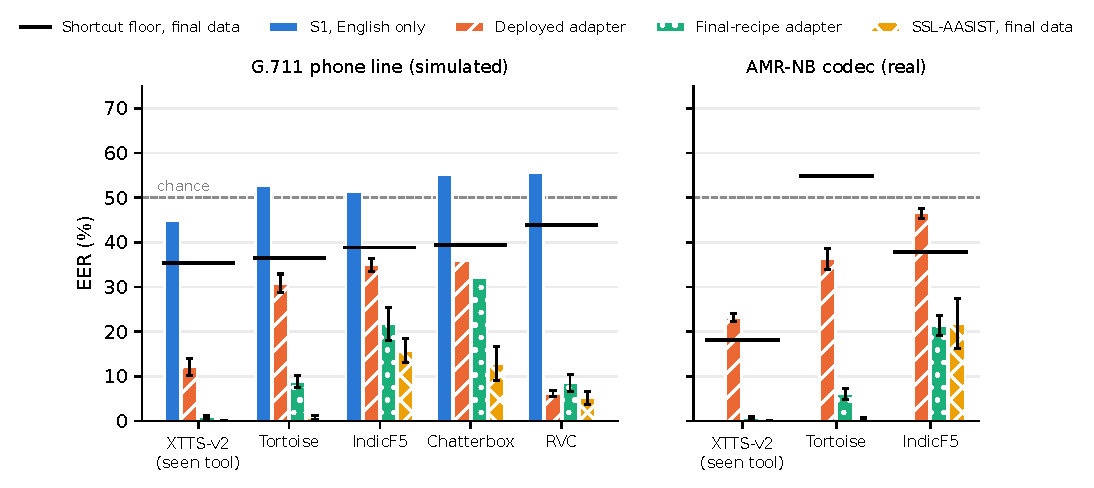
\includegraphics[width=\textwidth]{final_overview.pdf}
\caption{EER of the main systems on every attack tool, over the simulated G.711 line
(left) and the real AMR-NB codec (right; S1, at 40--50\% there, is not drawn). Bars are means over
five training seeds with one standard deviation; S1 and Chatterbox for both adapters are
one model each. The black tick is the shortcut floor fitted on the final training data, so
it applies to the two final-data systems only;
the dashed line is chance.}
\label{fig:overview}
\end{figure*}

\subsection{Outside baselines and a larger encoder}

Scored with their published weights, AASIST rejects 82.3\% of genuine Hindi--English
speech and SSL-AASIST 73.1\%, so the gap is not particular to our architecture. Fine-tuned
on the 248 speakers over G.711 (three seeds), AASIST beats our adapter trained on the same
data on Tortoise (CM04 16.7\% against 24.5\%,
$p = 0.036$) but loses on the seen tool (1.8\% against 0.9\%), on RVC (13.5\% against
6.5\%) and in false alarms (2.3\% against 0.5\%). On the seen tool, Tortoise and false
alarms both systems gain far more from the added voices than they differ from each other; on
IndicF5 AASIST barely moves, and its RVC error doubles.

SSL-AASIST, with about three times the parameters of our encoder, is the strongest system
once trained on the final-recipe data (Table~\ref{tab:final}). It is better than the
adapter in every seed on eight of eleven sets (Chatterbox, with one adapter seed, is not
counted), and reaches 0.51\% on new-speaker Tortoise over AMR-NB and 12.86\% on Chatterbox,
the adapter's hardest tool, where the adapter is at 31.98\% (one seed). It was not scored on
English.
It is fast enough for a live call: a 4~s window takes 69~ms on a T4 GPU and 1.14~s on two
CPU threads, inside the 2~s hop between windows. IndicF5 stays at 15.8--21.8\% for both
systems. Fig.~\ref{fig:overview} sets the main systems against every tool.

\section{The live-call system}

The deployed system runs the evaluation protocol on a live call (Fig.~\ref{fig:system}).
Two carriers, WebRTC for browser calls and Twilio Media Streams for the telephone network,
deliver 16~kHz mono audio to one shared detector. A streaming scorer takes a 4~s window
every 2~s, skips silence below $-50$~dBFS, normalises to $-23$~dBFS and scores on a worker
thread, so a slow window cannot stall the call. One window is too noisy to act on, so a
verdict ladder escalates only when consecutive windows agree: a caution after two
fake-leaning windows and ``likely cloned'', with a spoken warning, after four, with recovery
after three genuine-leaning ones. On speech this places the first caution near 6~s and the
spoken warning near 10~s. Verdicts
go only to the person receiving the call, because a caller who learns they have been
detected also learns how to evade the detector.

\begin{figure}[t]
\centering
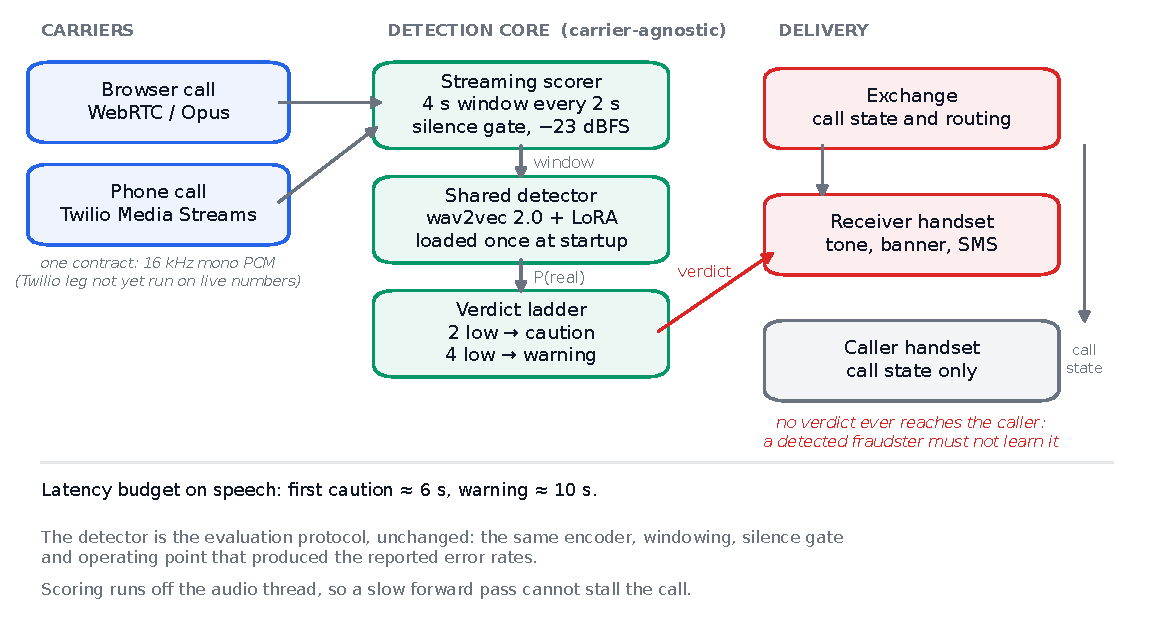
\includegraphics[width=\columnwidth]{system_architecture.pdf}
\caption{The live-call detector. Both carriers deliver the same 16~kHz mono audio, so the
detection core does not depend on the carrier. Verdicts reach only the receiver's handset.}
\label{fig:system}
\end{figure}

Table~\ref{tab:calls} shows what a caller meets. We replayed test clips through the live
scoring path and joined clips of one label into 60~s calls. The final recipe's threshold
was chosen on development calls only, by the rule used for the deployed model: the most
sensitive setting whose genuine calls raise at most 5\% alerts of any level (for the final
recipe, a caution after three fake-leaning windows and ``likely cloned'' after five). On read speech the final
recipe is the better live model. It no longer warns genuine new speakers (44\% of their
calls to none) and it catches every Tortoise call (33\% to 100\%), but it catches fewer
IndicF5 and Chatterbox calls, and every genuine spontaneous call is warned by either
model. The WebRTC carrier is verified end to end; the Twilio carrier is implemented
and unit-tested but has not yet run on live numbers.

\textbf{Real phone calls.} As a pilot, we made calls among ourselves, with written consent
and our faculty mentor's approval, over a commercial mobile network: 30 calls from the three
of us, twelve genuine live calls, six replays of our own readings from a laptop speaker, and
twelve replays of clones of our voices (XTTS-v2 and Chatterbox). The receiving handset
recorded each call, and we scored the recordings offline through the live scoring path after
a G.711 round trip, at each model's frozen threshold. The deployed model takes every replayed
call to ``likely cloned'', and eight of the twelve genuine live calls: all of two speakers'
and none of the third's. The final recipe warns three of twelve genuine live calls (one
``likely cloned''), all from one speaker, and takes five of six XTTS-v2 clone calls to
``likely cloned'' (for two speakers only 30--46~s into the call) and none of six Chatterbox
calls (it cautions one). Against the fair control, the genuine replays that share the
clones' loudspeaker path, one of six reaches ``likely cloned''. Rebuilding the call chain on
our direct recordings (Fig.~\ref{fig:realchain}) shows the real AMR-NB codec is the largest
step in the deployed model's failure: averaged over six readings its mean P(genuine) is 0.75
through the simulated line and 0.50 through AMR-NB (two readings cross the threshold there;
one was below it before any codec; the third speaker's two stay at 0.87--1.00), and 0.38
on the live calls. The final recipe stays above 0.8 at every stage; it adds more voices as
well as AMR-NB, which these calls cannot separate.

\begin{figure}[t]
\centering
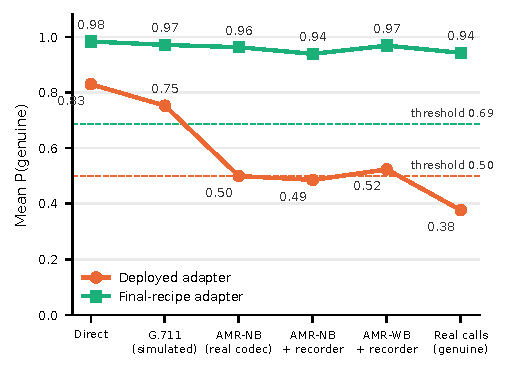
\includegraphics[width=\columnwidth]{real_call_chain.pdf}
\caption{Mean P(genuine) of our direct recordings through each stage of a phone call, and of
the genuine live calls as the carrier delivers them. Dashed: each model's live threshold.}
\label{fig:realchain}
\end{figure}

\begin{table}[t]
\centering
\caption{60~s calls through the live path: share of genuine calls warned and of fake calls
caught, each meaning a caution or worse. Counts are small (6--41 calls per cell).}
\label{tab:calls}
\small
\setlength{\tabcolsep}{4pt}
\begin{tabular}{@{}lrrrr@{}}
\toprule
 & \multicolumn{2}{c}{Genuine warned} & \multicolumn{2}{c}{Fakes caught} \\
Test calls & Depl. & Final & Depl. & Final \\
\midrule
Evaluation pool (XTTS) & 0\%   & 0\%   & 100\% & 100\% \\
CM04 (Tortoise)        & 0\%   & 0\%   & 33\%  & 100\% \\
RVC test half          & 0\%   & 0\%   & 100\% & 100\% \\
60 new speakers        & 44\%  & 0\%   & 100\% & 100\% \\
IndicF5                & 0\%   & 0\%   & 67\%  & 50\% \\
Chatterbox             & 0\%   & 0\%   & 33\%  & 17\% \\
HiACC, spontaneous     & 100\% & 100\% & --    & -- \\
\bottomrule
\end{tabular}
\end{table}

\section{Limitations}

\textbf{Unseen tools.} We have no conclusive evidence that the deployed model detects an
unseen tool over a phone line. The final recipe and SSL-AASIST do beat their floors, but
three of those floors are above chance, IndicF5 stays near 16--22\%, and Chatterbox is at
32\% for the adapter.

\textbf{Spontaneous speech.} All code-mixed training speech is read lectures. On HiACC, which
differs from them in both speaking style and recording, the deployed model calls 54.37\% of genuine spontaneous clips fake, against 0.89\% for read
lectures, and the final recipe 43.9\% (one seed, within the 38.5--54.4\% spread of single
trainings). Two SSL-AASIST trainings with equal development
scores call 5.8\% and 46.7\% of these clips fake, so the larger encoder can learn
spontaneous speech but does not do so reliably. Spontaneous genuine speech is needed in
training.

\textbf{English.} The deployed model is meant for Hindi--English calls. English passed
through the same channel rises to 24.20\% EER, against 6.50\% for S1. The final recipe
errs the other way: it rarely rejects genuine English but lets most English clones
through.

\textbf{Our attacks, our channel.} The attacks are of our own making, and most are not
hard: the seen tool sits half a MOS point below genuine speech. The channel is simulated,
with one real codec, and the real-call test is a pilot of 30 calls from the three authors.

\section{Conclusion}

An English-trained deepfake detector fails on Hindi--English telephone speech by rejecting
genuine speakers, and a language-controlled test shows that the cause is not code-mixing:
the gap follows the recording domain. A low-rank adapter that trains 1.13\% of the
parameters closes the gap on the seen tool and keeps clean English. More training speakers
and a real mobile codec close most of the remaining gap on the unseen Tortoise generator
without any of its audio in training, and a larger encoder fine-tuned on the same data goes
further. Spontaneous speech, the most natural generator we scored (IndicF5) and Chatterbox
remain open. We report each code-mixed EER of the systems we adapt against a matched shortcut
floor rather than against zero, and we suggest that results on
newly built corpora be read the same way.

\section*{Code and data availability}

The code, configurations, frozen speaker pools, manifests, generation job tables and
per-clip scores behind every number are in the project repository at the tag
\texttt{paper-v1}, with the seeds used. The cloned audio is not released, because it is
the speech of identifiable people; its metadata and checksums are. MUCS 2021 and HiACC are
available from their publishers.

% Acknowledgments go here once the team has agreed the wording (question 12).

\bibliographystyle{IEEEtran}
\bibliography{../refs}

\end{document}
